\documentclass[../TFG_Report.tex]{subfiles}
 
\begin{document}



\subsection{Airfoil selection}

In this section, the selection of the airfoils for the blades will be made. First, the desired characteristics will be defined. The low Reynolds influence will be described, and a study methodology will be chosen according to it. Then, several existing airfoils will be selected to be studied and a selection criteria will be detailed.Finally, the elected airfoil will be characterized. 


\subsubsection*{Desired characteristics}

The desired performance of the blades varies from root to tip. The optimal solution would be to have blades with aerodynamic twist and adapt the airfoil selection to the different circumstances of each section of the blade. However, this would difficult the optimization of the chord and geometric twist distribution, so only one airfoil will be selected. \\

This selection is a compromise between aerodynamic and structural issues. Usually, a high relative thickness is used at the root (around 35\%) and a lower one at the tip (18\%). The biggest drawback of a single-airfoil blade is that this could not be done. The desired characteristics of the airfoil are enumerated in the following list: \cite{Apunts} \cite{Wood}


\begin{enumerate}
	\item Good performance at low Reynolds number. 
	\item High efficiency $(C_l/C_d)_{max}$.
	\item Margin between optimal and critical conditions (stall angle of attack far from the optimal angle of attack to be resistant to perturbations)
	\item High lift coefficient: a higher lift coefficient would lead to a lower chord, resulting in less loads and costs.  
	\item Soft stall behaviour.
	\item Insensitive to dirt (turbulent airfoils are more resistant). 
\end{enumerate}

\subsubsection*{Low Reynolds number and simulation parameters }

The Reynolds number in a small wind turbine is defined as:

\begin{equation}
Re = \frac{\rho U_T c }{\mu}
\end{equation}

Where $U_T$ is the "total" velocity at the blade, $c$ is the chord, $\rho$ is the air density and $\mu$ the dynamic viscosity. Note that the first two variables change along the blade. Note that the lower Reynolds value will be achieved when the blades are stationary and $U_T = U_0$. The typical Re ranges for small wind turbines and other aerodynamic bodies can be found in the following table: 

\begin{figure}[h!]
	\centering
	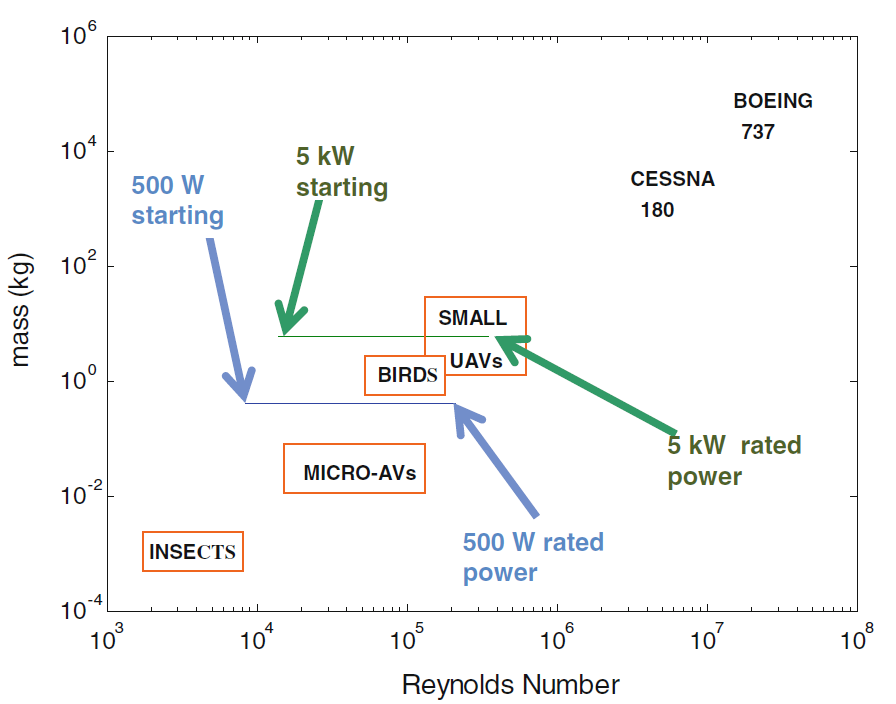
\includegraphics[width=0.6\linewidth]{Images/Low_RE_Number}
	\caption[Reynolds number ranges]{Reynolds number ranges for small wind turbines and other aerodynamic bodies. \\
		Obtained from \cite{Wood}.}
	\label{fig:LowReNumber}
\end{figure}

\FloatBarrier

The airfoils will be studied using XFOIL sofware with XFLR5 graphical user interface. As it uses an inviscid linear-vorticity panel method with a Karman-Tsien compressibility correction, this software shows reliable results for low Re flows. Note that it was initially intended for the calculation of model sailplanes. The following constant parameters need to be defined to set up the simulation \cite{fuentes2016airfoil}: 

\begin{enumerate}
	\item \textbf{Mach number}: As XFOIL considers incompressible flow (M=0) any value below 0.3, this value is initially defined as $M=0$.
	
	\item \textbf{Boundary layer transition}: It is assumed that the laminar to turbulent transition will occur due to the roughness of the blades. The XFOIL documentation is followed, and a value of Ncrit = 1 is set. \cite{XFOIL} 
		 
	\item \textbf{Reynolds number}: Although reliability can be expected from XFOIL results, the error increases at significant low Reynolds. The following Reynolds will be studied: $Re=2\cdot10^5$, $Re=1.6\cdot10^5$, $Re=1.2\cdot10^5$, $Re=8\cdot10^4$, and $Re=4\cdot10^4$.
\end{enumerate}



%It is known that lift and drag coefficients depend on the Reynolds number. Although computational analysis is very used for airfoil study, there are authors that state these results can not be completely trusted at low Re \cite{Wood}. There is also low accurate experimental data available for these cases ($Re<10^5$) due to the small forces involved. In order to reduce uncertainties and ensure veracity of the data used, this design will be limited to a little amount of well-studied airfoils designed specifically for small wind turbines. 

\subsubsection*{Airfoils studied}

The following table summarizes the airfoils that will be tested and studied. The airfoil coordinates and the values presented below has been obtained from \textit{airfoiltools.com} \cite{Airfoiltools}, a useful website that uses UIUC's airfoil database \cite{UIUC}. All the airfoils studied have been designed looking for a good performance in low Reynolds number operation. Some of them are specifically designed for small wind turbines: SG series (Selig-Giguere) and S833/4/5 airfoils designed by NREL are probably the first aerofoils designed for this purpose \cite{Wood}. The other models have been selected by looking into low Reynolds airfoils studies \cite{fuentes2016airfoil} \cite{shah2012low}.  

\begin{center}

	\rowcolors{4}{}{lightgray}
	\begin{longtable}{C{1cm}|C{2cm}|C{2.2cm}C{1.5cm}|C{2.2cm}C{1.5cm}}
	\caption[Airfoils selected to be studied.]{Airfoils selected to be studied. All values are indicated in chord percentage.}	\label{tab:Airfoils_Studied}  \\ 
	Code &	Airfoil & Maximum thickness [\%]& Position [\%]   & Maximum camber [\%]& Position  [\%]                                \\ \hline \endhead
	1&	SG6040  & 16.0           & 35.3                  & 2.3       & 60.5                \\
	2&	SG6041  & 10.0           & 34.9                 & 1.5       & 49.7                \\
	3&	SG6042  & 10.0           & 33.5                 & 3.3       & 51.5                \\
	4&	SG6043  & 10.0          & 32.1                  & 5.1       & 53.3               \\
	5&	S833    & 18.0           & 36.3                  & 2.5       & 78.8                  \\
	6&	S834    & 15.0           & 39.5                  & 1.6       & 60.0                    \\
	7&	S835    & 21.0           & 30.5                  & 2.4       & 78.0                   \\
	8&	S1210   &   12.0            &     21.4       &   6.7          &    51.1           \\
	9&	S1223   &   12.1          &     19.8          &     8.1        &  49.9               \\
	10&	S6063   &     7.0        &       29.4           &     1.3        &   43.8          \\
	11&	S9037   &     9.0        &    28.5              &   3.3    &       42.4          \\
	12&	S3010   &     10.3	     &  	25        &    2.3         &       43.3            \\
	13&	SD8000  &       8.9     &     29.4        &    1.5       &       54               \\
	14&	BW3     &      5.0           &      7.4        &    5.7         &    45.4             \\
	15&	E387    &      9.1        &      31.1       &     3.2        &    44.8           \\
	16&	E374    &    10.9         &    34.3         &    2.0       & 38.9             \\
	17&	E62     &     5.6            &       26.2       &     5.0        &      49.3         \\
	18&	RG15    &      8.9           &      30.2            &    1.8         &  39.7		
	\end{longtable}

\end{center}

\FloatBarrier

The following parameters will be analyzed for each airfoil:



\begin{enumerate}
	\item Maximum efficiency $E$: An airfoil that produces the more lift possible with the minimum drag is desired. 
	\item $\Delta \alpha=\alpha_{s}-\alpha_{opt}$: It is important to have the optimum angle of attack far from the stall angle of attack, as this provides consistency to the design. 
	\item $\dfrac{d\alpha_{opt}}{dRe}$: The Reynolds range that the airfoil will work at makes desirable to have uniformity in the optimal operating point. Hence, the lower variation of its location is searched. 
	\item $\dfrac{dE}{dRe}$: The same reason than the previous point. 
	\item $\dfrac{dE}{d \alpha} (\alpha=\alpha_{opt})$: This parameter is also studied in order to provide consistency. Variations of $\alpha$ should not lead to huge changes in the efficiency. 
	\item Thickness $t/c$: The thicker the airfoil, the more structural resistance it has. Usually the thicnkess is a compromise between the aerodynamic performance and the structural perspective. 
	\item $Cl_{opt}$: The higher the lift coefficient for, the smaller the chord needed.
	
\end{enumerate}

An explanation of how the data have been extracted from each airfoil can be found in the section \ref{RA_Aero_Design} of the Report Attachment. The polar curves and data from each airfoil is also presented there with more detail. The results are summarized in the following table: 


\begin{table}[]
	\centering
	\rowcolors{5}{}{lightgray}
		\caption{Airfoil selection results.}
	\label{tab:my-table}
	\begin{tabular}{cc|C{1.5cm}|C{1.5cm}|C{1.75cm}|C{1.5cm}|C{1.5cm}|C{1.5cm}|C{1.3cm}}
		&         & \multicolumn{7}{c}{Parameters}                                                      \\\cline{3-9}
		&         & 1     & 2       & 3                            & 4      & 5     & 6         & 7     \\ 
		\multirow{-3}{*}{Nº} & \multirow{-3}{*}{Airfoil}  & $E_{max}$ & $\alpha_{s}-\alpha_{opt}$ & $d\alpha_{opt}/dRe$ & $dE/dRe$ & $dE/d\alpha$ & $(t/c)_{max}$ & $Cl_{opt}$ \\ \hline
		1          & SG6040  & 44.11 & 10.81   & 0.55                         & 9.86   & 4.66  & 16.00     & 0.87  \\
		2          & SG6041  & 42.46 & 6.02    & 0.36                         & 7.50   & 2.14  & 10.00     & 0.89  \\
		3          & SG6042  & 48.89 & 9.24    & 0.64 & 8.01   & 2.57  & 10.00     & 0.85  \\
		4          & SG6043  & 57.73 & 10.96   & 0.94                         & 11.87  & 5.59  & 10.00     & 0.97  \\
		5          & S833    & 31.13 & 8.59    & 0.69                         & 6.32   & 1.32  & 18.00     & 0.75  \\
		6          & S834    & 32.30 & 7.62    & 0.33                         & 5.96   & 1.32  & 15.00     & 0.69  \\
		7          & S835    & 27.96 & 10.03   & 0.60                         & 6.00   & 1.97  & 21.00     & 0.67  \\
		8          & S1210   & 62.47 & 6.32    & 0.31                         & 12.13  & 4.80  & 12.00     & 1.40  \\
		9          & S1223   & 55.67 & 5.63    & 0.37                         & 10.55  & 1.44  & 12.10     & 1.52  \\
		10         & S6063   & 36.78 & 3.89    & 0.18                         & 5.36   & 5.57  & 7.00      & 0.67  \\
		11         & S9037   & 50.95 & 6.57    & 0.09                         & 8.55   & 2.33  & 9.00      & 0.93  \\
		12         & S3010   & 48.35 & 5.97    & 0.07                         & 8.59   & 2.45  & 10.30     & 0.94  \\
		13         & SD8000  & 42.76 & 5.35    & 0.06                         & 7.24   & 2.15  & 8.90      & 0.84  \\
		14         & BW3     & 45.99 & 6.27    & 0.49                         & 5.89   & 2.96  & 5.00      & 1.08  \\
		15         & E387    & 56.17 & 6.85    & 0.66                         & 10.42  & 9.22  & 9.10      & 0.89  \\
		16         & E374    & 44.81 & 7.98    & 0.56                         & 7.04   & 6.69  & 10.90     & 0.71  \\
		17         & E62     & 65.55 & 7.02    & 0.72                         & 11.70  & 13.64 & 5.60      & 0.95  \\
		18         & RG15    & 43.48 & 5.41    & 0.25                         & 6.74   & 4.66  & 8.90      & 1.83 
	\end{tabular}

\end{table}

In order to select which airfoil will be used, the preceding table should be normalized, and each parameter should have a weight assigned. A common risk when comparing different possibilities is to select an option which stands out in a particular variable but is not the best option in average. To avoid so, a domination matrix will be used \cite{ApuntsDomMatrix}. The matrices with normalization and the domination procedure may be found in the section \ref{RA_Airfoil_Decision} of the Report Attachment.


%FALTA POSAR BIBLIOGRAFIA DOMINATION MATRIX
%RESULTATS SELECCIÓ AIRFOIL
%EXPLICAR COM ÉS L'AIRFOIL TRIAT I CARACTERÍSTIQUES



\subsection{Blades design}

%FER INTRODUCCIÓ QUAN ESTIGUI TOT FET

In this section the whole aerodynamic design of the blades will be reviewed. Firstly, the method to compute the power curve of a given blade geometry will be described. After that, different methods to optimize it will be discussed, as well as the distinctive feature that this passive solution should take into account. 

%Explicar procediment: intersecció amb la corba del generador, algoritme genetic per maximitzar, codi massa lent (número de vegades que fa la BEM), simplement provar distribucions de corda i twist optima tenint en compte el Starting Time i la corda màxima. Càlcul aproximat per les unions


\subsubsection{Power curve calculation}

To be able to design the blade geometry, the first step is creating a code to obtain the power curve from a given chord, pitch and twist. These three will be the variables to be determined. With them, the goal is to maximize the Annual Energy Production (AEP) by means of the power curve. \\

If a generator is selected, the curve of torque vs rotor speed $Q=f(\Omega)$ is fixed. This curve will also be the one that the wind turbine will follow. With it, it is already know how much torque the rotor will have to produce at each rotational speed in order to match the generator demand and achieve an equilibrium point. The remaining task is to compute the at which wind speed these equilibrium points are obtained. If a $\Omega = f(U_{\infty})$ function can be found, then these points can be traced into a $Q=f(U_{\infty})$ function and the desired power curve $P=f(U_{\infty})$ would be immediate to obtain. In order to do so, the following procedure has been made: 


\begin{figure}[h!]
	\centering
	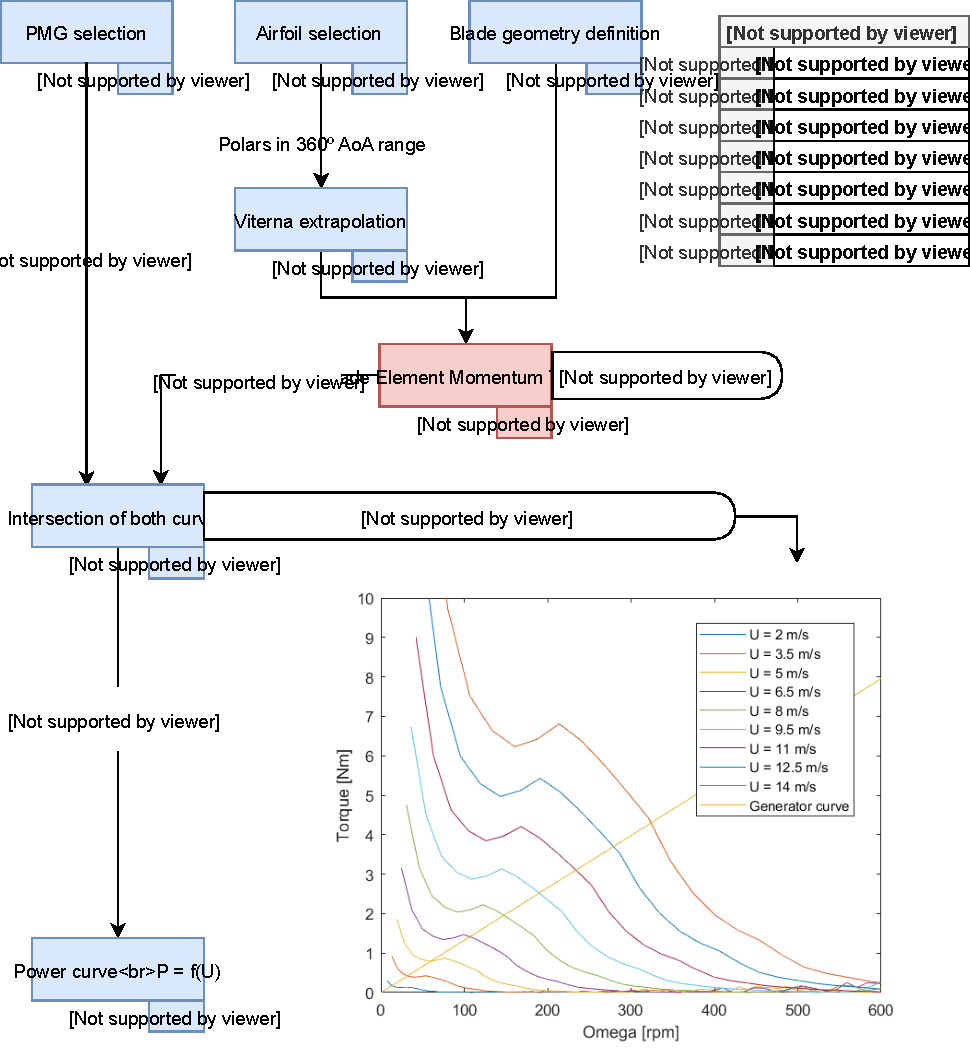
\includegraphics[width=1\linewidth]{Images/Power_curve_procedure_image}
	\caption[Power curve calculation procedure]{Power curve calculation procedure. Includes the Matlab function created for each step, so the code is easier to analyze.}
	\label{fig:PowerCurveScheme}
\end{figure}




\subsubsection{Initial approach and design challenge}\label{sec:design_challenge}

A first study was carried out in order to see the general behavior of the wind turbine, analyze trends, and start to delimit which blade geometry may be more beneficial. To do so, a big number of chord and twist distributions were simulated. The pitch was also included, but as there is not any kind of pitch control, it is treated as a static offset to the twist. \\

%Check GENERATOR SPEED!!!!!!!
The first consideration that should be taken into account is the fact that the wind turbine will be working at a very big RPM range. The generator has a nominal rotor speed of 600 RPM, whereas a typical commercial size wind turbine (e.g. General Electric - Cypress platform) works around 10 RPM. The dimensions of them are clearly not comparable, and the reference parameter should be the tip speed ratio. This will be the focus of this study and the source of the design challenge. \\

%Reference formulas to the Handbook!! Also explain how the formulas are obtained
Both the chord and twist distribution used were obtained using the analytic formulas proposed in the section 3.7.3. of the Wind Energy Handbook by T. Burton et al. \cite{Handbook}. These expressions are analytically obtained in order to have the optimum induction coefficients $a$ and $a'$ (and thus, maximizing the power coefficient $C_P$) for a given tip speed ratio $\lambda$. For obtaining these formulas no losses have been taken into account. Moreover, the drag has been ignored, although it is demonstrated in the section 3.7.4. of the Handbook that the effect of including it is indeed negligible.   %

\begin{equation}\label{OptimalChord}
c = R \dfrac{2 \pi}{\lambda N C_L} \dfrac{8/9}{\sqrt{4/9+(\lambda \mu)^2  \cdot \left( 1+\dfrac{2}{9 (\lambda \mu)^2 } \right)^2 }}
\end{equation}

\begin{equation}\label{OptimalTwist}
\beta = \phi - \alpha = \arctan{\left(   \dfrac{2/3}{\lambda \mu \left( 1+\dfrac{2}{9 (\lambda \mu)^2}   \right)}   \right)} -\alpha
\end{equation}

%Posar valors concrets?
The $\alpha$ is selected to get the maximum efficiency $C_L/C_D$, and the lift coefficient is given by it. For this step, this point is obtained with the average of all Reynolds number studied. The airfoil study showed that this airfoil has little angle of attack variation at different Reynolds numbers, so this selection is representative of all the operation region. For this study, different pitch variations (offset to the twist) have been applied. \\


To have a general sense of what the optimal blade geometry for this case will look like, the procedure shown in the preceding section has been applied to all the different chord and twist distributions. Then, the Annual Energy Production (AEP) has been calculated using a Weibull wind speed distribution. The Weibull used, due to the lack of experimental data of a possible installation site, corresponds to the reference one used in the Small Wind Turbine Contest \cite{SWTContest}: $A=4.5$ m/s ($V_{ave}=4.0$ m/s) and $k=2$. The blade geometry that lead to the higher AEP has been selected, and now its characteristics are going to be analyzed. \\

First, the chord and twist distribution of the selected blade geometry: 

\begin{figure}[h!]
	\centering
	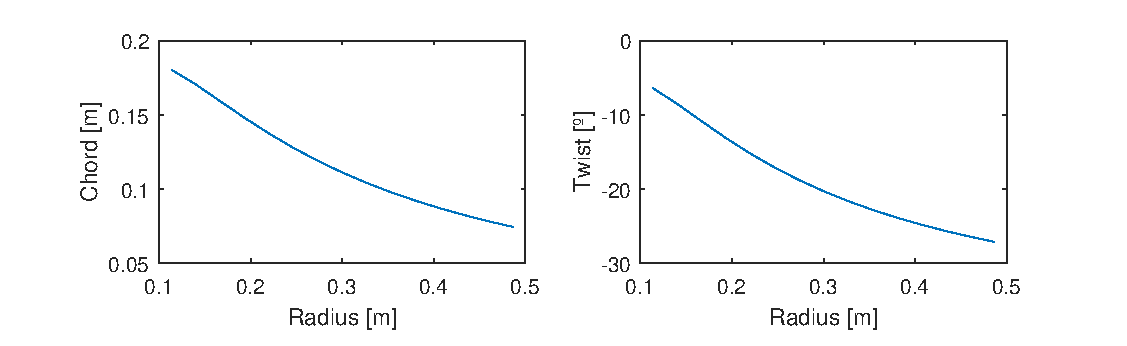
\includegraphics[width=1\linewidth]{Images/Aerodynamic_Design/First_Chord_Twist}
	\caption[First chord and twist distribution obtained]{First chord and twist distribution obtained. This distribution is optimized for a tip speed ratio of 2.8, and has a pitch offset of -36º.}
	\label{fig:ChordTwistFirst}
\end{figure}

\FloatBarrier

At first glance, it might seem abnormal the large pitch offset that is applied to the twist. The optimal twist distribution is created such that the effective angle of attack seen by the blades is always the optimal one $\alpha_{opt}$. Therefore, a big change like that is surprising. The explanation of why this is more beneficial from an AEP point of view will be developed after the presentation of these first results. \\

\begin{figure}[h!]
	\centering
	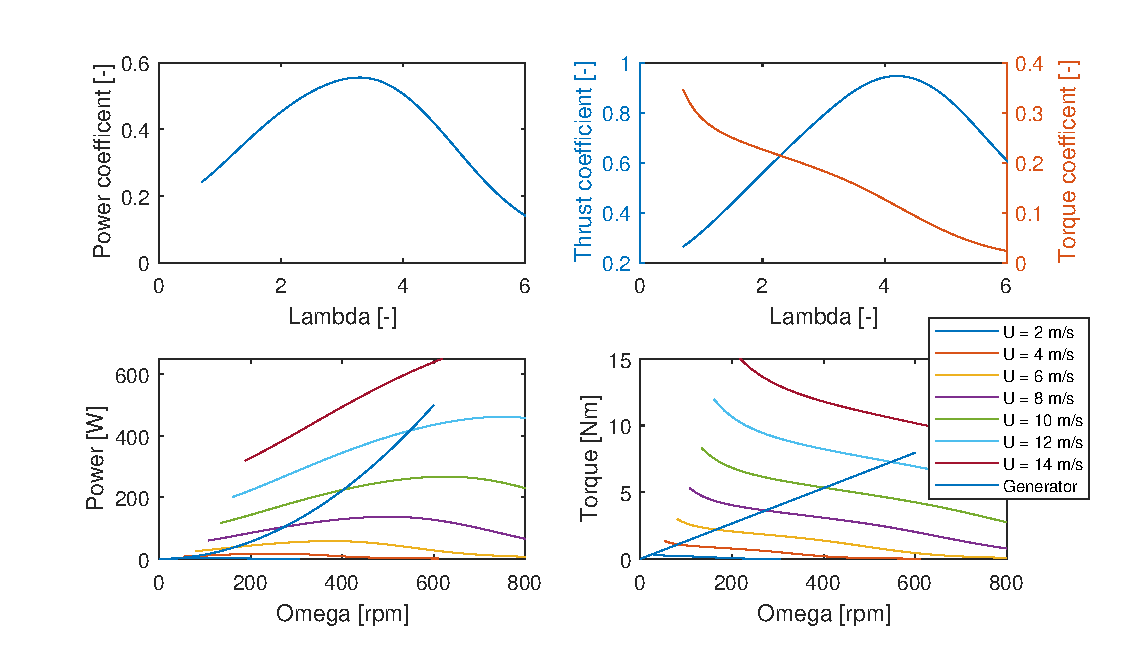
\includegraphics[width=1\linewidth]{Images/Aerodynamic_Design/First_Lambda_Results}
	\caption[Rotor coefficients as a function of lambda. Intersection with the generator curve. (first results)]{Rotor coefficients as a function of lambda and intersection with the generator curve. The bottom plots show both the generator (the curves that start at the origin of coordinates) and the rotor curves. The rotor curve is shown for different wind speeds and tip speed ratios. Each different curve is one wind speed, and each of its points corresponds to a different tip speed ratio.   }
	\label{fig:LambdaResultstFirst}
\end{figure}

\FloatBarrier

As it was explained in the preceding section (Figure \ref{fig:PowerCurveScheme}), the intersection of the rotor and the generator curve will give the operating points of the design. By doing so, the following power curve and operation are obtained.

\begin{figure}[h!]
	\centering
	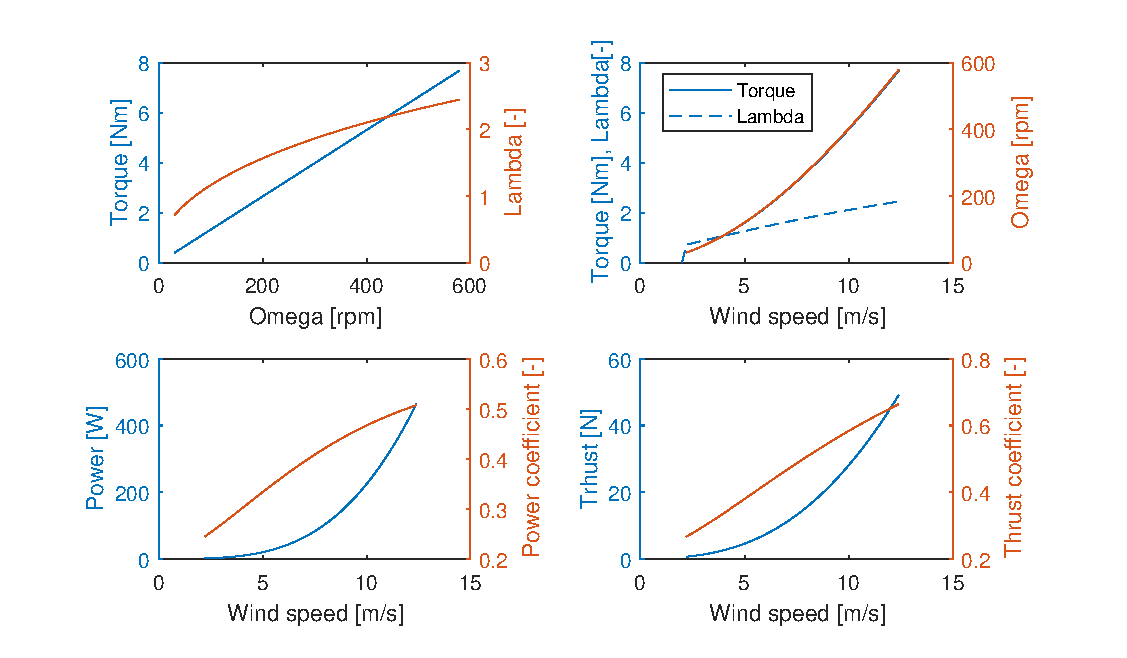
\includegraphics[width=1\linewidth]{Images/Aerodynamic_Design/First_Operation_Results}
	\caption[First operation results]{First operation results. }
	\label{fig:OperationResultstFirst}
\end{figure} 
 \FloatBarrier

The cut-in wind speed is the one at which the power extracted by the blades is enough to energize the generator. On the other hand, the cut-out wind speed is the wind speed such that the maximum generator power is reached. The region after that will be treated separately, because it will involve furling and big yaw misalignment, and these phenomena is not easy to study with the BEM theory. \\

The most important remark about the results obtained may be seen in the top right plot. The dashed blue lines shows the tip speed ratio $\lambda$ as function of the wind speed. Clearly there is a large variation from the cut-in (0.71) to the cut-out (2.44). It is interesting to note that this variation has been found not only in this design, but in all the different rotor geometries analyzed. This has an immediate effect on the angle of attack seen by the blades during all the operation. From the BEM (inherent definition of the induction factors) it is known that the angle of attack $\alpha$ can be obtained as follows: 

\begin{equation}
\alpha = \phi - \beta = \arctan\left(\dfrac{U_{\infty} (1-a)}{\Omega r (1+a')}   \right) - \beta = \arctan\left(\dfrac{(1-a)}{\lambda_r (1+a')}   \right) - \beta 
\end{equation}

The inverse tangent is a growing  function. Thus, if the tip speed ratio is increased, the fraction will decrease, and the angle of attack will decrease (as $\beta$, the sum of the twist and the pitch, is constant). This also depends on the induction factors $a$ and $a'$, but this explanation is enough to understand this effect, and the variation of these factors is more difficult to predict and study as they also depend on the tip speed ratio. The mean angle of attack as a function of the wind speed may be seen in the following figure.  

\begin{figure}[h!]
	\centering
	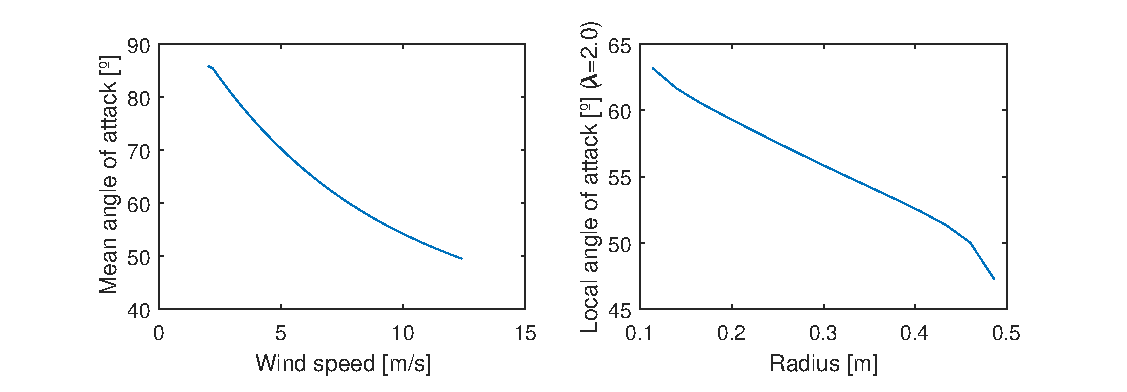
\includegraphics[width=1\linewidth]{Images/Aerodynamic_Design/First_AngleOfAttack_Analysis}
	\caption[Angle of attack variation of the first results]{Angle of attack variation of the first results. The left plot shows the mean angle of attack (of all sections) as a function of the incoming wind speed. The right one shows the local angle of attack for a given tip speed ratio ($\lambda=2$).  }
	\label{fig:AngleOfAttackAnalysisFirst}
\end{figure} 
\FloatBarrier

The large angle of attack variation anticipated is observed. The initial mean angle of attack is 85.6º, whereas at the cut-out wind speed is less than 50º. There is a change of more than 40º during all the operation curve. Then, the main question to be asked is: why a design like that appears to be the optimal one? It is surprising that the working region of the airfoils is outside the linear zone. In order to find out an explanation, the airfoil polar can be plotted once again: \\

\begin{figure}[h!]
	\centering
	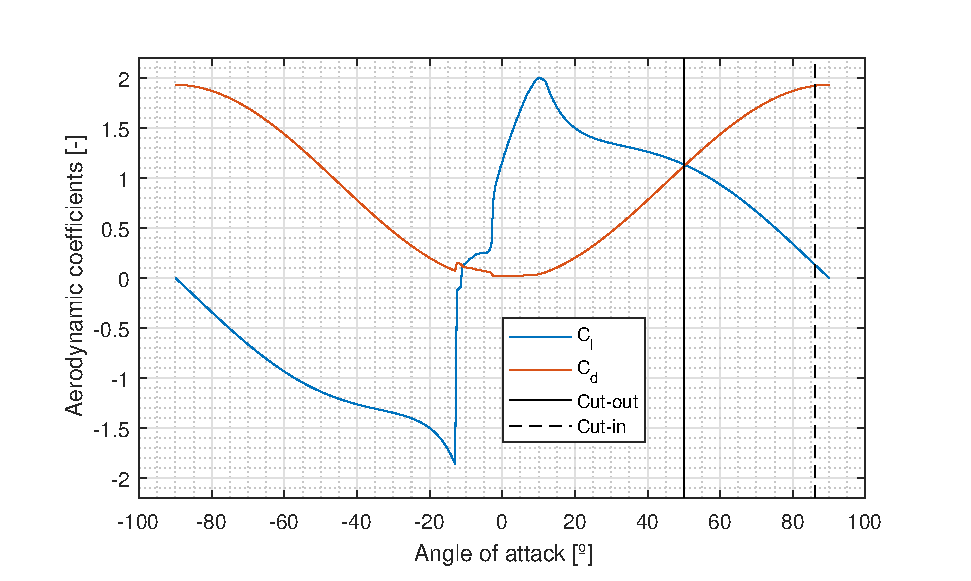
\includegraphics[width=1\linewidth]{Images/Aerodynamic_Design/First_Polars_OpRegion}
	\caption[]{Airfoil polar with operation region indicated.}
	\label{fig:AngleOfAttackPolarsFirst}
\end{figure} 
\FloatBarrier

To understand why this operation is more beneficial, firstly it could be analyzed what would happen if the operation regime was located in the linear region. If the cut-in mean angle of attack were, for example, 20º, and the cut-out one were -20º, almost the half of the operation would have a negative lift coefficient. The BEM equations from which the axial induction factor is obtained may show the effect that this has: 

%FIXAR-SE SI AIXÒ JA S'HA EXPLICAT EN UN ALTRE LLOC I REFERENCIAR-HO!!!!
\begin{equation}
C_l \cos \phi + C_d \sin \phi = C_x
\end{equation}


\begin{equation}
\dfrac{a}{1-a} = \dfrac{\sigma_r}{4 \sin^2\phi} C_x
\end{equation}

The coefficient of sectional blade element force normal to the rotor plane $C_x$ would be negative in that case, therefore the axial induction factor $a$ would be less than zero as well. It should be constrained between 0 and 1, so this possibility cannot be studied with the BEM theory without reversing the rotational direction. It makes no sense to reverse the direction in the middle of the operation. Moreover, an operation like that would not match the generator curve, so it would not be possible.   \\

On the other hand, if the operation is contained in the region obtained, the lift coefficient variation is more stable. Furthermore, its value near the cut-out region (where the power produced is higher) is also larger, which is an advantage from a power coefficient point of view. It could be argued that operating from 60º to 20º, for example, would be more beneficial, because the operation would be as solid as the obtained one, and the lift coefficient values would be higher. Firstly, the influence of the flow angle $\phi$ should be taken into account with more detail, and secondly, the number of blade geometries tested was low (225), so it is likely that no geometry capable to operate at that regime was created. Nevertheless, this first study was intended to understand the design challenge that will be faced, as well as the general operating characteristics of the design, and this result is enough for that. \\

An operation like this is not viable. The post stall region is very stochastic, unstable, and it could easily lead to high vibrations and aeroelastic instabilities. The drag is also unacceptable there. However, the behavior seen here is also obtained in other blade geometries analyzed, so it must be taken into consideration for further design. This performance could be summarized as follows: decrease of the angle of attack and increase of the tip speed ratio from the cut-in to the cut-out. It is also interesting to note that a stall control could not be implemented. A typical stall regulated wind turbine works in a constant rotor speed. As the tip speed ratio is defined as $\lambda = \Omega R / U_{\infty}$, as the wind speed increases, the tip speed ratio decreases, and it has been demonstrated that a lower tip speed ratio leads to a higher angle of attack. If it is design properly, the stall will be reached at the desired wind speed. 


%%Coses que s'han vist:
	%-Gran regim de lambda, gran regim AoA. En alguns casos surt millor treballar en la regió de post-stall (foto)
	%-Cut out quan s'acaba la intersecció -> Si Weibull es petita, no val la pena operar més enllà d'aquella U
	%-Operem a lambdes baixes però la pala està optimizada amb lambda més gran (per la chord solidity i corda massa gran a l'arrel). Farem aproximació linel





\subsubsection{Optimization procedure}









	
	



	
\end{document}